\documentclass[../main/NEMO_manual]{subfiles}

\begin{document}

\chapter{Lateral Boundary Condition (LBC)}
\label{chap:LBC}

\chaptertoc

\paragraph{Changes record} ~\\

{\footnotesize
  \begin{tabularx}{\textwidth}{l||X|X}
    Release & Author(s) & Modifications \\
    \hline
    {\em  next} & {\em Simon M{\" u}ller} & {\em Minor update of \autoref{subsec:LBC_bdy_tides}} \\[2mm]
    {\em   4.0} & {\em ...} & {\em ...} \\
    {\em   3.6} & {\em ...} & {\em ...} \\
    {\em   3.4} & {\em ...} & {\em ...} \\
    {\em <=3.4} & {\em ...} & {\em ...}
  \end{tabularx}
}

\clearpage

\cmtgm{Add here introduction to this chapter}

%% =================================================================================================
\section[Boundary condition at the coast (\forcode{rn_shlat})]{Boundary condition at the coast (\protect\np{rn_shlat}{rn\_shlat})}
\label{sec:LBC_coast}

\begin{listing}
  \nlst{namlbc}
  \caption{\forcode{&namlbc}}
  \label{lst:namlbc}
\end{listing}

%The lateral ocean boundary conditions contiguous to coastlines are Neumann conditions for heat and salt
%(no flux across boundaries) and Dirichlet conditions for momentum (ranging from free-slip to "strong" no-slip).
%They are handled automatically by the mask system (see \autoref{subsec:DOM_msk}).

%OPA allows land and topography grid points in the computational domain due to the presence of continents or islands,
%and includes the use of a full or partial step representation of bottom topography.
%The computation is performed over the whole domain, \ie\ we do not try to restrict the computation to ocean-only points.
%This choice has two motivations.
%Firstly, working on ocean only grid points overloads the code and harms the code readability.
%Secondly, and more importantly, it drastically reduces the vector portion of the computation,
%leading to a dramatic increase of CPU time requirement on vector computers.
%The current section describes how the masking affects the computation of the various terms of the equations
%with respect to the boundary condition at solid walls.
%The process of defining which areas are to be masked is described in \autoref{subsec:DOM_msk}.

Options are defined through the \nam{lbc}{lbc} namelist variables.
The discrete representation of a domain with complex boundaries (coastlines and bottom topography) leads to
arrays that include large portions where a computation is not required as the model variables remain at zero.
Nevertheless, vectorial supercomputers are far more efficient when computing over a whole array,
and the readability of a code is greatly improved when boundary conditions are applied in
an automatic way rather than by a specific computation before or after each computational loop.
An efficient way to work over the whole domain while specifying the boundary conditions,
is to use multiplication by mask arrays in the computation.
A mask array is a matrix whose elements are $1$ in the ocean domain and $0$ elsewhere.
A simple multiplication of a variable by its own mask ensures that it will remain zero over land areas.
Since most of the boundary conditions consist of a zero flux across the solid boundaries,
they can be simply applied by multiplying variables by the correct mask arrays,
\ie\ the mask array of the grid point where the flux is evaluated.
For example, the heat flux in the \textbf{i}-direction is evaluated at $u$-points.
Evaluating this quantity as,

\[
  % \label{eq:LBC_aaaa}
  \frac{A^{lT} }{e_1 }\frac{\partial T}{\partial i}\equiv \frac{A_u^{lT}
  }{e_{1u} } \; \delta_{i+1 / 2} \left[ T \right]\;\;mask_u
\]
(where mask$_{u}$ is the mask array at a $u$-point) ensures that the heat flux is zero inside land and
at the boundaries, since mask$_{u}$ is zero at solid boundaries which in this case are defined at $u$-points
(normal velocity $u$ remains zero at the coast) (\autoref{fig:LBC_uv}).

\begin{figure}[h]
  \centering
  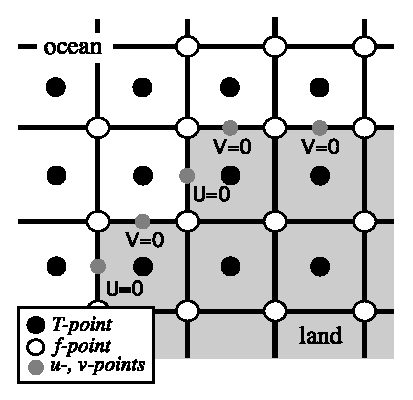
\includegraphics[width=0.33\textwidth]{LBC_uv}
  \caption[Lateral boundary at $T$-level]{
    Lateral boundary (thick line) at T-level.
    The velocity normal to the boundary is set to zero.}
  \label{fig:LBC_uv}
\end{figure}

For momentum the situation is a bit more complex as two boundary conditions must be provided along the coast
(one each for the normal and tangential velocities).
The boundary of the ocean in the C-grid is defined by the velocity-faces.
For example, at a given $T$-level,
the lateral boundary (a coastline or an intersection with the bottom topography) is made of
segments joining $f$-points, and normal velocity points are located between two $f-$points (\autoref{fig:LBC_uv}).
The boundary condition on the normal velocity (no flux through solid boundaries)
can thus be easily implemented using the mask system.
The boundary condition on the tangential velocity requires a more specific treatment.
This boundary condition influences the relative vorticity and momentum diffusive trends,
and is required in order to compute the vorticity at the coast.
Four different types of lateral boundary condition are available,
controlled by the value of the \np{rn_shlat}{rn\_shlat} namelist parameter
(The value of the mask$_{f}$ array along the coastline is set equal to this parameter).
These are:

\begin{figure}[h]
  \centering
  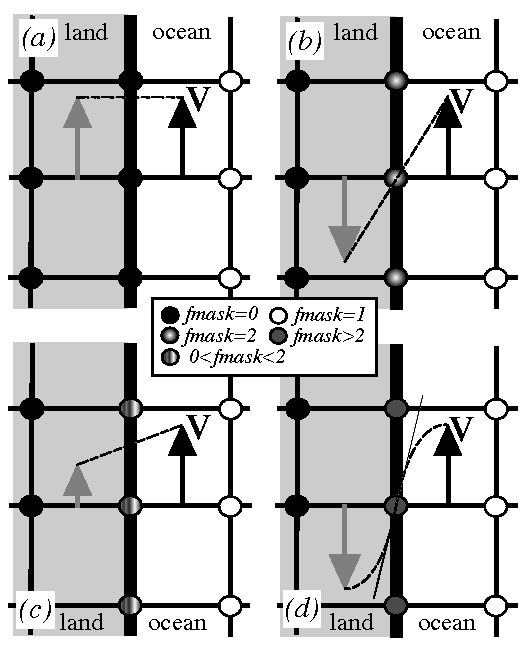
\includegraphics[width=0.33\textwidth]{LBC_shlat}
  \caption[Lateral boundary conditions]{
    Lateral boundary conditions
    (a) free-slip                       (\protect\np[=0]{rn_shlat}{rn\_shlat});
    (b) no-slip                         (\protect\np[=2]{rn_shlat}{rn\_shlat});
    (c) "partial" free-slip (\forcode{0<}\protect\np[<2]{rn_shlat}{rn\_shlat}) and
    (d) "strong" no-slip    (\forcode{2<}\protect\np{rn_shlat}{rn\_shlat}).
    Implied "ghost" velocity inside land area is display in grey.}
  \label{fig:LBC_shlat}
\end{figure}

\begin{description}

\item [free-slip boundary condition ({\np[=0]{rn_shlat}{rn\_shlat}})] the tangential velocity at
  the coastline is equal to the offshore velocity,
  \ie\ the normal derivative of the tangential velocity is zero at the coast,
  so the vorticity: mask$_{f}$ array is set to zero inside the land and just at the coast
  (\autoref{fig:LBC_shlat}-a).

\item [no-slip boundary condition ({\np[=2]{rn_shlat}{rn\_shlat}})] the tangential velocity vanishes at the coastline.
  Assuming that the tangential velocity decreases linearly from
  the closest ocean velocity grid point to the coastline,
  the normal derivative is evaluated as if the velocities at the closest land velocity gridpoint and
  the closest ocean velocity gridpoint were of the same magnitude but in the opposite direction
  (\autoref{fig:LBC_shlat}-b).
  Therefore, the vorticity along the coastlines is given by:

  \[
    \zeta \equiv 2 \left(\delta_{i+1/2} \left[e_{2v} v \right] - \delta_{j+1/2} \left[e_{1u} u \right] \right) / \left(e_{1f} e_{2f} \right) \ ,
  \]
  where $u$ and $v$ are masked fields.
  Setting the mask$_{f}$ array to $2$ along the coastline provides a vorticity field computed with
  the no-slip boundary condition, simply by multiplying it by the mask$_{f}$ :
  \[
    % \label{eq:LBC_bbbb}
    \zeta \equiv \frac{1}{e_{1f} {\kern 1pt}e_{2f} }\left( {\delta_{i+1/2}
        \left[ {e_{2v} \,v} \right]-\delta_{j+1/2} \left[ {e_{1u} \,u} \right]}
    \right)\;\mbox{mask}_f
  \]

\item ["partial" free-slip boundary condition (0$<$\np{rn_shlat}{rn\_shlat}$<$2)] the tangential velocity at
  the coastline is smaller than the offshore velocity, \ie\ there is a lateral friction but
  not strong enough to make the tangential velocity at the coast vanish (\autoref{fig:LBC_shlat}-c).
  This can be selected by providing a value of mask$_{f}$ strictly inbetween $0$ and $2$.

\item ["strong" no-slip boundary condition (2$<$\np{rn_shlat}{rn\_shlat})] the viscous boundary layer is assumed to
  be smaller than half the grid size (\autoref{fig:LBC_shlat}-d).
  The friction is thus larger than in the no-slip case.

\end{description}

Note that when the bottom topography is entirely represented by the $s$-coordinates (pure $s$-coordinate),
the lateral boundary condition on tangential velocity is of much less importance as
it is only applied next to the coast where the minimum water depth can be quite shallow.

%% =================================================================================================
\section{Model domain boundary condition}
\label{sec:LBC_jperio}

At the model domain boundaries several choices are offered:
closed, cyclic east-west, cyclic north-south, a north-fold, and combination closed-north fold or
bi-cyclic east-west and north-fold.
The north-fold boundary condition is associated with the 3-pole ORCA mesh.

%% =================================================================================================
\subsection{Closed, cyclic (\forcode{l_Iperio,l_Jperio})}
\label{subsec:LBC_jperio012}

The choice of closed or cyclic model domain boundary condition is controled by
setting the internal code variables \forcode{l_Iperio,l_Jperio} to true or false.
The way these variables are defined will differ accoring to the value of \np{ln_read_cfg}{ln\_read\_cfg} parameter in
namelist \nam{cfg}{cfg}, which usage is detailed in \autoref{subsec:DOM_config}. If \np[=.false.]{ln_read_cfg}{ln\_read\_cfg} the user must define \forcode{l_Iperio,l_Jperio} trough the routine \mdl{usrdef\_nam}. If \np[=.true.]{ln_read_cfg}{ln\_read\_cfg}, \forcode{l_Iperio,l_Jperio} will be defined according to the values of the global attributes (\texttt{Iperio,Jperio} = 0 or 1) in the NetCDF domain configuration file defined by \np{cn_domcfg}{cn\_domcfg} parameter in namelist \nam{cfg}{cfg}.
Each time such a boundary condition is needed, it is set by a call to routine \rou{lbc\_lnk} routine (found in \mdl{lbclnk} module).

\begin{description}

\item [For closed boundary (\forcode{l_Iperio = .false.,l_Jperio = .false.})], solid walls are imposed at all model boundaries: first and last rows and columns the the domain must be set to zero and will be forced to 0 if nedeed.

\item [For cyclic east-west boundary (\forcode{l_Iperio = .true.,l_Jperio = .false.})], first and last rows are set to zero (closed). The first \np{nn_hls}{nn\_hls} columns (left side halo) are defined with the last \np{nn_hls}{nn\_hls} columns of the orginal global domain (without halos). The last \np{nn_hls}{nn\_hls} columns (right side halo) are defined with the first \np{nn_hls}{nn\_hls} columns of the orginal global domain (without halos). Whatever flows out of the eastern (western) end of the basin enters the western (eastern) end.

\item [For cyclic north-south boundary (\forcode{l_Iperio = .false.,l_Jperio = .true.})], first and last columns are set to zero (closed). Whatever flows out of the northern (southern) end of the basin enters the southern (northern) end.

\item [Bi-cyclic east-west and north-south boundary (\forcode{l_Iperio = .true.,l_Jperio = .true.})] combines cases 1 and 2.

\end{description}

\begin{figure}[!t]
  \centering
  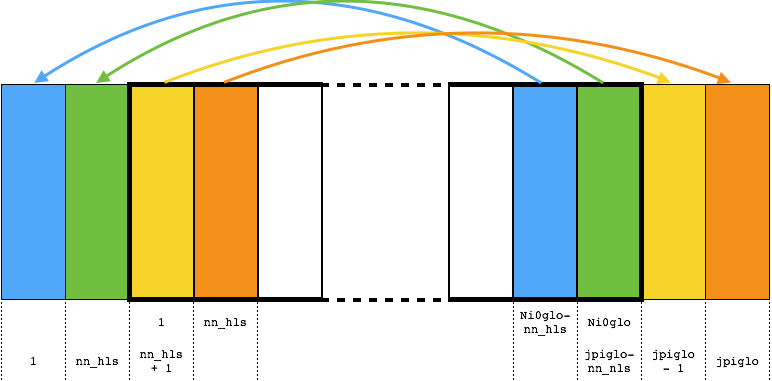
\includegraphics[width=0.5\textwidth]{LBC_Iperio}
  \caption{Setting of east-west cyclic boundary conditions for \np[=2]{nn_hls}{nn\_hls}. The orginal global domain (without halos) is delimited by the thick lines.}
  \label{fig:LBC_Iperio}
\end{figure}

%% =================================================================================================
\subsection{North-fold (\forcode{l_NFold = .true.})}
\label{subsec:LBC_north_fold}

The north fold boundary condition has been introduced in order to handle the north boundary of
a three-polar ORCA grid.
Such a grid has two poles in the northern hemisphere (\autoref{fig:CFGS_ORCA_msh},
and thus requires a specific treatment to ensure the proper boundary conditions at the northern edge of the domain.
Further information can be found in \autoref{apdx:NFOLD} and in \mdl{lbcnfd} module which applies the north fold boundary condition.

%% =================================================================================================
\section[Exchange with neighbouring processes (\textit{lbclnk.F90}, \textit{lib\_mpp.F90})]{Exchange with neighbouring processes (\protect\mdl{lbclnk}, \protect\mdl{lib\_mpp})}
\label{sec:LBC_mpp}

\begin{listing}
  \nlst{nammpp}
  \caption{\forcode{&nammpp}}
  \label{lst:nammpp}
\end{listing}

For massively parallel processing (mpp), a horizontal domain decomposition method is used, see \autoref{fig:LBC_3x3}.
The basic idea of the method is to split the large computation domain of a numerical experiment into several smaller domains and solve the set of equations by addressing independent local problems.
Each process has its own local memory and computes the model equation over a subdomain of the whole model domain.
The present implementation is largely inspired by Guyon's work [Guyon 1995].

\begin{figure}[h]
  \centering
  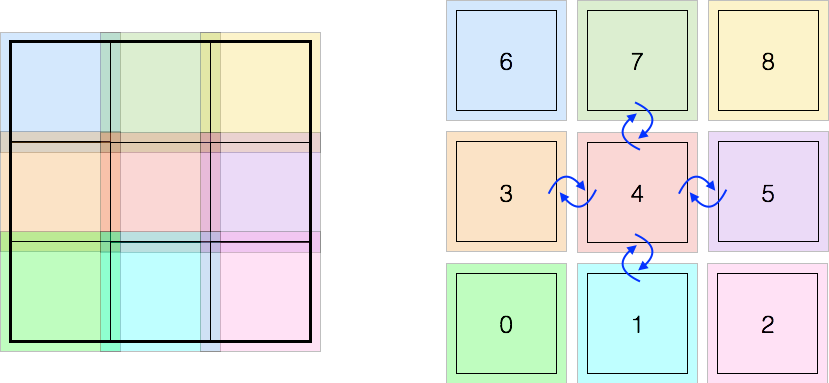
\includegraphics[width=0.66\textwidth]{LBC_3x3}
  \caption{Horizontal domain decomposition in $3 \times 3$ subdomains. The thick line on the left panel delimits the original domain (without halos). Subdomains numbering starts at 1 from the bottom-left subdomain, as shown on the right panel. Communications of the subdomain 4 with its neighbours are represented by the blue arrows.}
  \label{fig:LBC_3x3}
\end{figure}

Each subdomain computes its own inner subdomain. The subdomain boundary conditions, also called halos, are overlapping with neighbouring subdomains as show on the left panel of \autoref{fig:LBC_3x3}. The \rou{lbc\_lnk} routine (found in \mdl{lbclnk} module) is next used to fill the halos either by doing a communication with a neighbour or locally by applying a cyclic or closed boundary condition. The halos, consist of \np{nn_hls}{nn\_hls} (namelist \nam{mpp}{mpp}) rows/columns at each side of the subdomain.

When doing a communication, a process sends to its neighbouring processes the update values of the points corresponding to
the interior overlapping area to its neighbouring sub-domain (\ie\ the \np{nn_hls}{nn\_hls} innermost of the 2*\np{nn_hls}{nn\_hls} overlapping rows/columns, see blue arrows in \autoref{fig:LBC_3x3}).
The communication is done through the Message Passing Interface (MPI) which is activated by default since NEMO 4.2.
Use \key{mpi\_off} if MPI is not available on your computer or use \key{mpi2} if the MPI version of your computer is older than v3.
From the NEMO 4.2 release, a new communication strategy has been introduced to preserve performance efficiency
by reducing communication time, namely the MPI3 neighborhood collective communications.
It provides a way to have sub-communicators used to perform collective communications only among neighborhood.
A single MPI message is needed to be built for all neighbours instead of 4 different messages before calling the collective.
The new communication approach can be selected by setting the value of \np{nn_comm}{nn\_comm} parameter, defined in \nam{mpp}{mpp} namelist. \np[=1]{nn_comm}{nn\_comm} activates the point to point communications that was originally coded in NEMO and further optimized in NEMO 4.2. \np[=2]{nn_comm}{nn\_comm} selects the new collective communications.
The output file \textit{communication\_report.txt} provides the list of which routines do how
many communications during 1 time step of the model.

In \NEMO, the splitting is regular and arithmetic.
The total number of subdomains corresponds to the number of MPI processes allocated to \NEMO\ when the model is launched
(\ie\ mpirun -np x ./nemo will automatically give x subdomains).
The i-axis is divided by \np{jpni}{jpni} and the j-axis by \np{jpnj}{jpnj}.
These parameters are defined in \nam{mpp}{mpp} namelist.
If \np{jpni}{jpni} and \np{jpnj}{jpnj} are < 1, they will be automatically redefined in the code to give the best domain decomposition see bellow and \citep{Irrmann2022}. 

\begin{figure}[h]
  \centering
  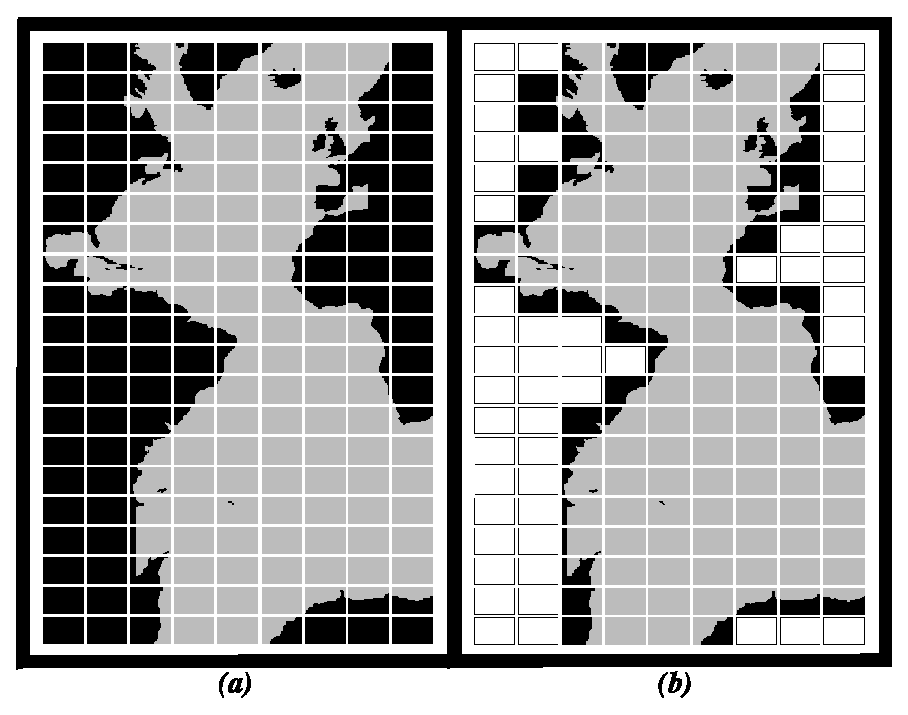
\includegraphics[width=0.66\textwidth]{LBC_mppini2}
  \caption[Atlantic domain defined for the CLIPPER projet]{
    Example of Atlantic domain defined for the CLIPPER projet.
    Initial grid is composed of 773 x 1236 horizontal points.
    (a) the domain is split onto 9 $times$ 20 subdomains (jpni=9, jpnj=20). Subdomains with ocean points are numbered first starting from bottom-left. The 52 subdomains that are land areas are next numbered starting also from bottom-left (in yellow).
    (b) The 52 subdomains are eliminated (white rectangles) and
    the resulting number of processors really used during the computation is 128. Note that the subdomains with ocean points have the same number in both cases.}
  \label{fig:LBC_mppini2}
\end{figure}

The \NEMO\ model computes equation terms with the help of mask arrays (0 on land points and 1 on sea points). It is therefore possible that an MPI subdomain contains only land points, see \autoref{fig:LBC_mppini2}. To save ressources, we try to supress from the computational domain as much land subdomains as possible. For example if $N_{mpi}$ processes are allocated to NEMO, the domain decomposition will be given by the following equation:
\[
  N_{mpi} = jpni \times jpnj - N_{land} + N_{useless}
\]
$N_{land}$ is the total number of land subdomains in the domain decomposition defined by \np{jpni}{jpni} and \np{jpnj}{jpnj}. $N_{useless}$ is the number of land subdomains that are kept in the compuational domain in order to make sure that $N_{mpi}$ MPI processes are indeed allocated to a given subdomain. The values of $N_{mpi}$, \np{jpni}{jpni}, \np{jpnj}{jpnj},  $N_{land}$ and $N_{useless}$ are printed in the output file \texttt{ocean.output}. $N_{useless}$ must, of course, be as small as possible to limit the waste of ressources. A warning is issued in  \texttt{ocean.output} if $N_{useless}$ is not zero. Note that non-zero value of $N_{useless}$ is uselly required when using AGRIF as, up to now, the parent grid and each of the child grids must use all the $N_{mpi}$ processes.

If the domain decomposition is automatically defined (when \np{jpni}{jpni} and \np{jpnj}{jpnj} are < 1), the decomposition chosen by the model will minimise the horizontal subdomain size (defined as $max_{all domains}(subdomain size)$) and maximize the number of eliminated land subdomains. This means that no other domain decomposition (a set of \np{jpni}{jpni} and \np{jpnj}{jpnj} values) will use less processes than $(jpni  \times  jpnj - N_{land})$ and get a smaller subdomain size.
In order to specify $N_{mpi}$ properly (minimize $N_{useless}$), you must run the model once with \np{ln_list}{ln\_list} activated. In this case, the model will start the initialisation phase, print the list of optimum decompositions ($N_{mpi}$, \np{jpni}{jpni} and \np{jpnj}{jpnj}) in \texttt{ocean.output} and directly abort. The maximum value of $N_{mpi}$ tested in this list is given by $max(N_{MPI\_tasks}, jpni \times jpnj)$. For example, run NEMO on 1 process with \np[=.true.]{ln_listonly}{ln\_listonly}, \np[=1000]{jpni}{jpni} and \np[=1]{jpnj}{jpnj} will print the list of optimum domains decomposition from 1 to about 10000.

Processors are numbered from 0 to $N_{mpi} - 1$. Subdomains containning some ocean points are numbered first from 0 to $jpni * jpnj - N_{land} -1$, starting from the bottom-left subdomains, see \autoref{fig:LBC_mppini2}. The remaining $N_{useless}$ land subdomains are numbered next starting from bottom-left (yellow numbers in \autoref{fig:LBC_mppini2}a), which means that, for a given (\np{jpni}{jpni}, \np{jpnj}{jpnj}), the numbers attributed to he ocean subdomains do not vary with $N_{useless}$.

When land processors are eliminated, the value corresponding to these locations in the model output files is undefined. \np{ln_mskland}{ln\_mskland} must be activated in order avoid Not a Number values in output files. Note that it is better to not eliminate land processors when creating a meshmask file (\ie\ when setting a non-zero value to \np{nn_msh}{nn\_msh}).


\begin{figure}[h]
  \centering
  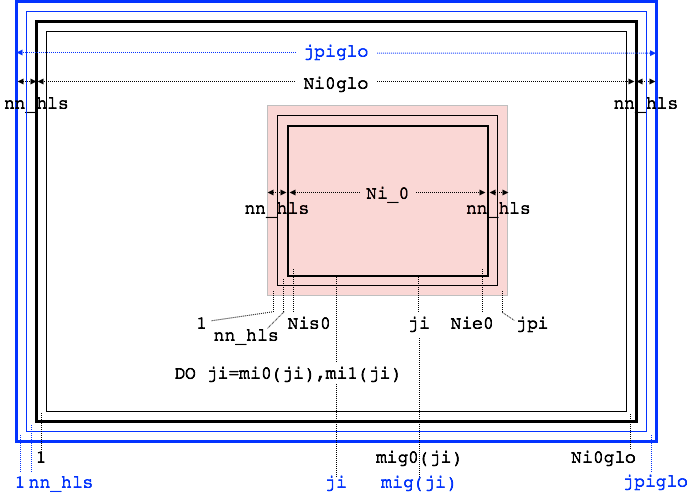
\includegraphics[width=0.66\textwidth]{LBC_mpp}
  \caption{Positioning of a sub-domain when massively parallel processing is used}
  \label{fig:LBC_mpp}
\end{figure}

Each processor is independent and without message passing or synchronous process, programs run alone and access just its own local memory. For this reason, the main model dimensions are the local dimensions of the subdomain that are named \forcode{jpi}, \forcode{jpj}, \forcode{jpk}. As detailed in \citet{Irrmann2022}, \forcode{jpi} and \forcode{jpj} can differ between subdomains. Note that if the configuration requires the North Pole folding (\forcode{l_NFold} = .True.), \forcode{jpj} of the processes involved in the folding is minimized in order to compensate the extra coast of the North Pole folding.
As show in \autoref{fig:LBC_mpp}, \forcode{jpi} and \forcode{jpj} include the inner or internal domain and the overlapping rows/columns. \forcode{Nis0} and \forcode{Nie0} are use to specify the inner domain.

As detailed in \autoref{fig:LBC_mpp}, several variables are defined to address indices from the local subdomain and the global domain (with or without halos). The whole domain dimensions are named \forcode{jpiglo}, \forcode{jpjglo} and \forcode{jpk}. \forcode{Ni0glo} and \forcode{Ni0glo} correspond to the original domain size, as seen in the input and output files, without any halo. The 1-d arrays $mig(1:jpi)$ and $mjg(1:jpj)$, defined in \rou{init\_locglo} routine (\mdl{mppini} module), should be used to get global domain (with halos) indices from local domain indices. An element of $T_{l}$, a local array (subdomain) corresponds to an element of $T_{g}$, a global array (whole domain including halos) by the relationship:
\[
  % \label{eq:LBC_nimpp}
  T_{g} (mig(i),mjg(j),k) = T_{l} (i,j,k),
\]
with $1 \leq i \leq jpi$, $1  \leq j \leq jpj $ , and  $1  \leq k \leq jpk$.
The 1-d arrays $mig0(1:jpi)$ and $mjg0(1:jpj)$ are used to get original global domain (without halos) indices from local domain indices. The 1-d arrays, $mi0(1:jpiglo)$, $mi1(1:jpiglo)$ and $mj0(1:jpjglo)$, $mj1(1:jpjglo)$ have the reverse purpose and should be used to define loop indices expressed in global domain indices (see examples in \mdl{dtastd} module).\\


%% =================================================================================================
\section{Unstructured open boundary conditions (BDY)}
\label{sec:LBC_bdy}

\begin{listing}
  \nlst{nambdy}
  \caption{\forcode{&nambdy}}
  \label{lst:nambdy}
\end{listing}

\begin{listing}
  \nlst{nambdy_dta}
  \caption{\forcode{&nambdy_dta}}
  \label{lst:nambdy_dta}
\end{listing}

Options are defined through the \nam{bdy}{bdy} and \nam{bdy_dta}{bdy\_dta} namelist variables.
The BDY module is the core implementation of open boundary conditions for regional configurations on
ocean temperature, salinity, barotropic-baroclinic velocities, ice-snow concentration, thicknesses, temperatures, salinity and melt ponds concentration and thickness.

The BDY module was modelled on the OBC module (see \NEMO\ 3.4) and shares many features and
a similar coding structure \citep{chanut_trpt05}.
The specification of the location of the open boundary is completely flexible and
allows any type of setup, from regular boundaries to irregular contour (it includes the possibility to set an open boundary able to follow an isobath).
Boundary data files used with versions of \NEMO\ prior to Version 3.4 may need to be re-ordered to work with this version.
See the section on the Input Boundary Data Files for details.

%% =================================================================================================
\subsection{Namelists}
\label{subsec:LBC_bdy_namelist}

The BDY module is activated by setting \np[=.true.]{ln_bdy}{ln\_bdy} .
It is possible to define more than one boundary ``set'' and apply different boundary conditions to each set.
The number of boundary sets is defined by \np{nb_bdy}{nb\_bdy}.
Each boundary set can be either defined as a series of straight line segments directly in the namelist
(\np[=.false.]{ln_coords_file}{ln\_coords\_file}, and a namelist block \forcode{&nambdy_index} must be included for each set) or read in from a file (\np[=.true.]{ln_coords_file}{ln\_coords\_file}, and a ``\textit{coordinates.bdy.nc}'' file must be provided).
The coordinates.bdy file is analagous to the usual \NEMO\ ``\textit{coordinates.nc}'' file.
In the example above, there are two boundary sets, the first of which is defined via a file and
the second is defined in the namelist.
For more details of the definition of the boundary geometry see section \autoref{subsec:LBC_bdy_geometry}.

For each boundary set a boundary condition has to be chosen for the barotropic solution
(``u2d'':sea-surface height and barotropic velocities), for the baroclinic velocities (``u3d''),
for the active tracers \footnote{The BDY module does not deal with passive tracers at this version} (``tra''), and for sea-ice (``ice'').
For each set of variables one has to choose an algorithm and the boundary data (set resp. by \np{cn_tra}{cn\_tra} and \np{nn_tra_dta}{nn\_tra\_dta} for tracers).\\

The choice of algorithm is currently as follows:

\begin{description}
\item [\forcode{'none'}:] No boundary condition applied.
  So the solution will ``see'' the land points around the edge of the edge of the domain.
\item [\forcode{'specified'}:] Specified boundary condition applied (only available for baroclinic velocity and tracer variables).
\item [\forcode{'neumann'}:] Value at the boundary are duplicated (No gradient). Only available for baroclinic velocity and tracer variables.
\item [\forcode{'frs'}:] Flow Relaxation Scheme (FRS) available for all variables.
\item [\forcode{'Orlanski'}:] Orlanski radiation scheme (fully oblique) for barotropic, baroclinic and tracer variables.
\item [\forcode{'Orlanski_npo'}:] Orlanski radiation scheme for barotropic, baroclinic and tracer variables.
\item [\forcode{'flather'}:] Flather radiation scheme for the barotropic variables only.
\end{description}

The boundary data is either set to initial conditions
(\np[=0]{nn_tra_dta}{nn\_tra\_dta}) or forced with external data from a file (\np[=1]{nn_tra_dta}{nn\_tra\_dta}).
In case the 3d velocity data contain the total velocity (ie, baroclinic and barotropic velocity),
the bdy code can derived baroclinic and barotropic velocities by setting \np[=.true.]{ln_full_vel}{ln\_full\_vel}
For the barotropic solution there is also the option to use tidal harmonic forcing either by
itself (\np[=2]{nn_dyn2d_dta}{nn\_dyn2d\_dta}) or in addition to other external data (\np[=3]{nn_dyn2d_dta}{nn\_dyn2d\_dta}).\\
If not set to initial conditions, sea-ice salinity, temperatures and melt ponds data at the boundary can either be read in a file or defined as constant (by \np{rn_ice_sal}{rn\_ice\_sal}, \np{rn_ice_tem}{rn\_ice\_tem}, \np{rn_ice_apnd}{rn\_ice\_apnd}, \np{rn_ice_hpnd}{rn\_ice\_hpnd}). Ice age is constant and defined by \np{rn_ice_age}{rn\_ice\_age}.

If external boundary data is required then the \nam{bdy_dta}{bdy\_dta} namelist must be defined.
One \nam{bdy_dta}{bdy\_dta} namelist is required for each boundary set, adopting the same order of indexes in which the boundary sets are defined in nambdy.
In the example given, two boundary sets have been defined. The first one is reading data file in the \nam{bdy_dta}{bdy\_dta} namelist shown above
and the second one is using data from intial condition (no namelist block needed).
The boundary data is read in using the fldread module,
so the \nam{bdy_dta}{bdy\_dta} namelist is in the format required for fldread.
For each required variable, the filename, the frequency of the files and
the frequency of the data in the files are given.
Also whether or not time-interpolation is required and whether the data is climatological (time-cyclic) data.
For sea-ice salinity, temperatures and melt ponds, reading the files are skipped and constant values are used if filenames are defined as {'NOT USED'}.\\

There is currently an option to vertically interpolate the open boundary data onto the native grid at run-time.
If \np{nn_bdy_jpk}{nn\_bdy\_jpk}$<-1$, it is assumed that the lateral boundary data are already on the native grid.
However, if \np{nn_bdy_jpk}{nn\_bdy\_jpk} is set to the number of vertical levels present in the boundary data,
a bilinear interpolation onto the native grid will be triggered at runtime.
For this to be successful the additional variables: $gdept$, $gdepu$, $gdepv$, $e3t$, $e3u$ and $e3v$, are required to be present in the lateral boundary files.
These correspond to the depths and scale factors of the input data,
the latter used to make any adjustment to the velocity fields due to differences in the total water depths between the two vertical grids.\\

In the example of given namelists, two boundary sets are defined.
The first set is defined via a file and applies FRS conditions to temperature and salinity and
Flather conditions to the barotropic variables. No condition specified for the baroclinic velocity and sea-ice.
External data is provided in daily files (from a large-scale model).
Tidal harmonic forcing is also used.
The second set is defined in a namelist.
FRS conditions are applied on temperature and salinity and climatological data is read from initial condition files.

%% =================================================================================================
\subsection{Flow relaxation scheme}
\label{subsec:LBC_bdy_FRS_scheme}

The Flow Relaxation Scheme (FRS) \citep{davies_QJRMS76,engedahl_T95},
applies a simple relaxation of the model fields to externally-specified values over
a zone next to the edge of the model domain.
Given a model prognostic variable $\Phi$
\[
  % \label{eq:LBC_bdy_frs1}
  \Phi(d) = \alpha(d)\Phi_{e}(d) + (1-\alpha(d))\Phi_{m}(d)\;\;\;\;\; d=1,N
\]
where $\Phi_{m}$ is the model solution and $\Phi_{e}$ is the specified external field,
$d$ gives the discrete distance from the model boundary and
$\alpha$ is a parameter that varies from $1$ at $d=1$ to a small value at $d=N$.
It can be shown that this scheme is equivalent to adding a relaxation term to
the prognostic equation for $\Phi$ of the form:
\[
  % \label{eq:LBC_bdy_frs2}
  -\frac{1}{\tau}\left(\Phi - \Phi_{e}\right)
\]
where the relaxation time scale $\tau$ is given by a function of $\alpha$ and the model time step $\Delta t$:
\[
  % \label{eq:LBC_bdy_frs3}
  \tau = \frac{1-\alpha}{\alpha}  \,\rdt
\]
Thus the model solution is completely prescribed by the external conditions at the edge of the model domain and
is relaxed towards the external conditions over the rest of the FRS zone.
The application of a relaxation zone helps to prevent spurious reflection of
outgoing signals from the model boundary.

The function $\alpha$ is specified as a $tanh$ function:
\[
  % \label{eq:LBC_bdy_frs4}
  \alpha(d) = 1 - \tanh\left(\frac{d-1}{2}\right),       \quad d=1,N
\]
The width of the FRS zone is specified in the namelist as \np{nn_rimwidth}{nn\_rimwidth}.
This is typically set to a value between 8 and 10.

%% =================================================================================================
\subsection{Flather radiation scheme}
\label{subsec:LBC_bdy_flather_scheme}

The \citet{flather_JPO94} scheme is a radiation condition on the normal,
depth-mean transport across the open boundary.
It takes the form
\begin{equation}
  \label{eq:LBC_bdy_fla1}
  U = U_{e} + \frac{c}{h}\left(\eta - \eta_{e}\right),
\end{equation}
where $U$ is the depth-mean velocity normal to the boundary and $\eta$ is the sea surface height,
both from the model.
The subscript $e$ indicates the same fields from external sources.
The speed of external gravity waves is given by $c = \sqrt{gh}$, and $h$ is the depth of the water column.
The depth-mean normal velocity along the edge of the model domain is set equal to
the external depth-mean normal velocity,
plus a correction term that allows gravity waves generated internally to exit the model boundary.
Note that the sea-surface height gradient in \autoref{eq:LBC_bdy_fla1} is a spatial gradient across the model boundary,
so that $\eta_{e}$ is defined on the $T$ points with $nbr=1$ and $\eta$ is defined on the $T$ points with $nbr=2$.
$U$ and $U_{e}$ are defined on the $U$ or $V$ points with $nbr=1$, \ie\ between the two $T$ grid points.

%% =================================================================================================
\subsection{Orlanski radiation scheme}
\label{subsec:LBC_bdy_orlanski_scheme}

The Orlanski scheme is based on the algorithm described by \citep{marchesiello.mcwilliams.ea_OM01}, hereafter MMS.

The adaptive Orlanski condition solves a wave plus relaxation equation at the boundary:
\begin{equation}
  \label{eq:LBC_wave_continuous}
  \frac{\partial\phi}{\partial t} + c_x \frac{\partial\phi}{\partial x} + c_y \frac{\partial\phi}{\partial y} =
  -\frac{1}{\tau}(\phi - \phi^{ext})
\end{equation}

where $\phi$ is the model field, $x$ and $y$ refer to the normal and tangential directions to the boundary respectively, and the phase
velocities are diagnosed from the model fields as:

\begin{equation}
  \label{eq:LBC_cx}
  c_x = -\frac{\partial\phi}{\partial t}\frac{\partial\phi / \partial x}{(\partial\phi /\partial x)^2 + (\partial\phi /\partial y)^2}
\end{equation}
\begin{equation}
  \label{eq:LBC_cy}
  c_y = -\frac{\partial\phi}{\partial t}\frac{\partial\phi / \partial y}{(\partial\phi /\partial x)^2 + (\partial\phi /\partial y)^2}
\end{equation}

(As noted by MMS, this is a circular diagnosis of the phase speeds which only makes sense on a discrete grid).
Equation (\autoref{eq:LBC_wave_continuous}) is defined adaptively depending on the sign of the phase velocity normal to the boundary $c_x$.
For $c_x$ outward, we have

\begin{equation}
\tau = \tau_{out}
\end{equation}

For $c_x$ inward, the radiation equation is not applied:

\begin{equation}
  \label{eq:LBC_tau_in}
  \tau = \tau_{in}\,\,\,;\,\,\, c_x = c_y = 0
\end{equation}

Generally the relaxation time scale at inward propagation points (\np{rn_time_dmp}{rn\_time\_dmp}) is set much shorter than the time scale at outward propagation
points (\np{rn_time_dmp_out}{rn\_time\_dmp\_out}) so that the solution is constrained more strongly by the external data at inward propagation points.
See \autoref{subsec:LBC_bdy_relaxation} for detailed on the spatial shape of the scaling.\\
The ``normal propagation of oblique radiation'' or NPO approximation (called \forcode{'orlanski_npo'}) involves assuming
that $c_y$ is zero in equation (\autoref{eq:LBC_wave_continuous}), but including
this term in the denominator of equation (\autoref{eq:LBC_cx}). Both versions of the scheme are options in BDY. Equations
(\autoref{eq:LBC_wave_continuous}) - (\autoref{eq:LBC_tau_in}) correspond to equations (13) - (15) and (2) - (3) in MMS.\\

%% =================================================================================================
\subsection{Relaxation at the boundary}
\label{subsec:LBC_bdy_relaxation}

In addition to a specific boundary condition specified as \np{cn_tra}{cn\_tra} and \np{cn_dyn3d}{cn\_dyn3d}, relaxation on baroclinic velocities and tracers variables are available.
It is control by the namelist parameter \np{ln_tra_dmp}{ln\_tra\_dmp} and \np{ln_dyn3d_dmp}{ln\_dyn3d\_dmp} for each boundary set.

The relaxation time scale value (\np{rn_time_dmp}{rn\_time\_dmp} and \np{rn_time_dmp_out}{rn\_time\_dmp\_out}, $\tau$) are defined at the boundaries itself.
This time scale ($\alpha$) is weighted by the distance ($d$) from the boundary over \np{nn_rimwidth}{nn\_rimwidth} cells ($N$):

\[
  \alpha = \frac{1}{\tau}(\frac{N+1-d}{N})^2,       \quad d=1,N
\]

The same scaling is applied in the Orlanski damping.

%% =================================================================================================
\subsection{Boundary geometry}
\label{subsec:LBC_bdy_geometry}

Each open boundary set is defined as a list of points.
The information is stored in the arrays $nbi$, $nbj$, and $nbr$ in the $idx\_bdy$ structure.
The $nbi$ and $nbj$ arrays define the local $(i,j)$ indexes of each point in the boundary zone and
the $nbr$ array defines the discrete distance from the boundary: $nbr=1$ means that
the boundary point is next to the edge of the model domain, while $nbr>1$ means that
the boundary point is increasingly further away from the edge of the model domain.
A set of $nbi$, $nbj$, and $nbr$ arrays is defined for each of the $T$, $U$ and $V$ grids.
\autoref{fig:LBC_bdy_geom} shows an example of an irregular boundary.

The boundary geometry for each set may be defined in a namelist \forcode{&nambdy_index} or
by reading in a ``\textit{coordinates.bdy.nc}'' file.
The \forcode{&nambdy_index} namelist defines a series of straight-line segments for north, east, south and west boundaries.
One \forcode{&nambdy_index} namelist block is needed for each boundary condition defined by indexes.
For the northern boundary, \texttt{nbdysegn} gives the number of segments,
\texttt{jpjnob} gives the $j$ index for each segment and \texttt{jpindt} and
\texttt{jpinft} give the start and end $i$ indices for each segment with similar for the other boundaries.
These segments define a list of $T$ grid points along the outermost row of the boundary ($nbr\,=\, 1$).
The code deduces the $U$ and $V$ points and also the points for $nbr\,>\, 1$ if \np[>1]{nn_rimwidth}{nn\_rimwidth}.

The boundary geometry may also be defined from a ``\textit{coordinates.bdy.nc}'' file.
\autoref{fig:LBC_nc_header} gives an example of the header information from such a file, based on the description of geometrical setup given above.
The file should contain the index arrays for each of the $T$, $U$ and $V$ grids.
The arrays must be in order of increasing $nbr$.
Note that the $nbi$, $nbj$ values in the file are global values and are converted to local values in the code.
Typically this file will be used to generate external boundary data via interpolation and so
will also contain the latitudes and longitudes of each point as shown.
However, this is not necessary to run the model.

For some choices of irregular boundary the model domain may contain areas of ocean which
are not part of the computational domain.
For example, if an open boundary is defined along an isobath, say at the shelf break,
then the areas of ocean outside of this boundary will need to be masked out.
This can be done by reading a mask file defined as \np{cn_mask_file}{cn\_mask\_file} in the nam\_bdy namelist.
Only one mask file is used even if multiple boundary sets are defined.

\begin{figure}[!t]
  \centering
  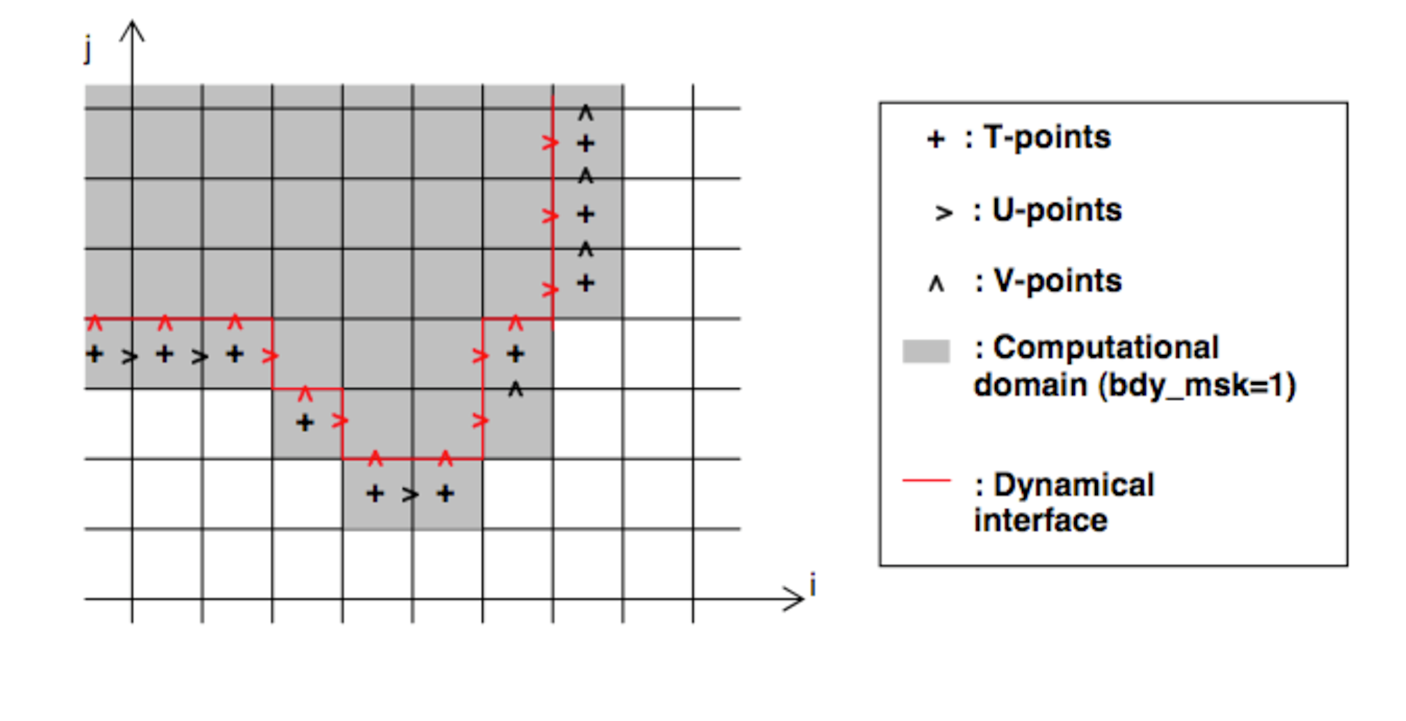
\includegraphics[width=0.66\textwidth]{LBC_bdy_geom}
  \caption[Geometry of unstructured open boundary]{Example of geometry of unstructured open boundary}
  \label{fig:LBC_bdy_geom}
\end{figure}

%% =================================================================================================
\subsection{Input boundary data files}
\label{subsec:LBC_bdy_data}

The data files contain the data arrays in the order in which the points are defined in the $nbi$ and $nbj$ arrays.
The data arrays are dimensioned on:
a time dimension;
$xb$ which is the index of the boundary data point in the horizontal;
and $yb$ which is a degenerate dimension of 1 to enable the file to be read by the standard \NEMO\ I/O routines.
The 3D fields also have a depth dimension.

From Version 3.4 there are new restrictions on the order in which the boundary points are defined
(and therefore restrictions on the order of the data in the file).
In particular:

\begin{enumerate}
\item The data points must be in order of increasing $nbr$,
  ie. all the $nbr=1$ points, then all the $nbr=2$ points etc.
\item All the data for a particular boundary set must be in the same order.
  (Prior to 3.4 it was possible to define barotropic data in a different order to
  the data for tracers and baroclinic velocities).
\end{enumerate}

These restrictions mean that data files used with versions of the
model prior to Version 3.4 may not work with Version 3.4 onwards.
A \fortran\ utility {\itshape bdy\_reorder} exists in the TOOLS directory which
will re-order the data in old BDY data files.

\begin{figure}[!t]
  \centering
  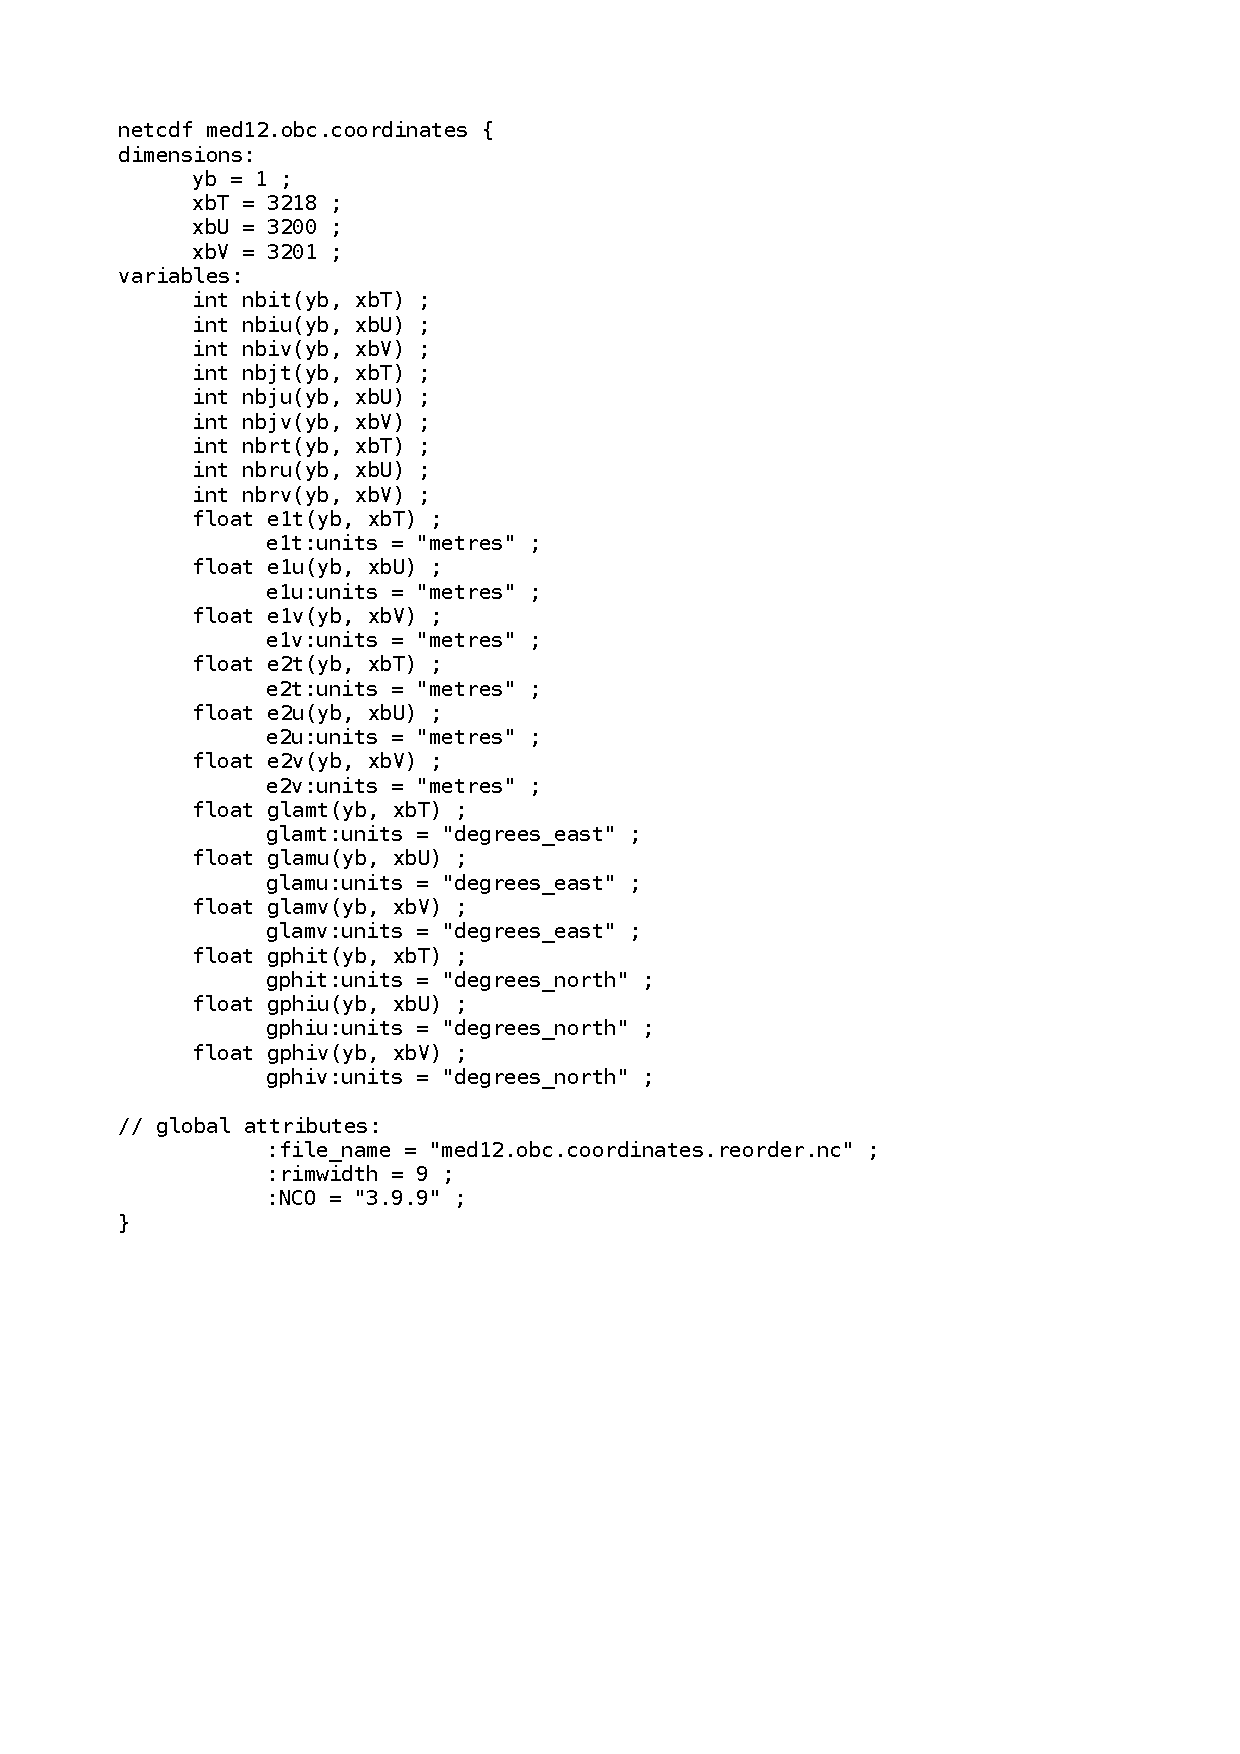
\includegraphics[width=0.66\textwidth]{LBC_nc_header}
  \caption[Header for a \textit{coordinates.bdy.nc} file]{
    Example of the header for a \textit{coordinates.bdy.nc} file}
  \label{fig:LBC_nc_header}
\end{figure}

%% =================================================================================================
\subsection{Volume correction}
\label{subsec:LBC_bdy_vol_corr}

There is an option to force the total volume in the regional model to be constant.
This is controlled  by the \np{ln_vol}{ln\_vol} parameter in the namelist.
A value of \np[=.false.]{ln_vol}{ln\_vol} indicates that this option is not used.
Two options to control the volume are available (\np{nn_volctl}{nn\_volctl}).
If \np[=0]{nn_volctl}{nn\_volctl} then a correction is applied to the normal barotropic velocities around the boundary at
each timestep to ensure that the integrated volume flow through the boundary is zero.
If \np[=1]{nn_volctl}{nn\_volctl} then the calculation of the volume change on
the timestep includes the change due to the freshwater flux across the surface and
the correction velocity corrects for this as well.

If more than one boundary set is used then volume correction is
applied to all boundaries at once.

%% =================================================================================================
\subsection{Tidal harmonic forcing}
\label{subsec:LBC_bdy_tides}

\begin{listing}
  \nlst{nambdy_tide}
  \caption{\forcode{&nambdy_tide}}
  \label{lst:nambdy_tide}
\end{listing}

Tidal forcing at open boundaries requires the activation of surface
tides (i.e., in \nam{_tide}{\_tide}, \np[=.true.]{ln_tide}{ln\_tide} with the active tidal
constituents listed in the \np{sn_tide_cnames}{sn\_tide\_cnames} array; see
\autoref{sec:SBC_TDE}). The specific options related to the reading in of
the complex harmonic amplitudes of elevation (SSH) and barotropic
velocity components (u,v) at the open boundaries are defined through the
\nam{bdy_tide}{bdy\_tide} namelist parameters.\par

The tidal harmonic data at open boundaries can be specified in two
different ways, either on a two-dimensional grid covering the entire
model domain or along open boundary segments; these two variants can
be selected by setting \np[=.true.]{ln_bdytide_2ddta}{ln\_bdytide\_2ddta} or
\np[=.false.]{ln_bdytide_2ddta}{ln\_bdytide\_2ddta}, respectively. In either
case, the real and imaginary parts of SSH, u, and v amplitudes associated with
each activated tidal constituent \texttt{<constituent>} have to be provided
separately as fields in input files with names based on
\np[=<input>]{filtide}{filtide}: when two-dimensional data is used, variables
\texttt{<constituent>\_z1} and \texttt{<constituent>\_z2} for the real and imaginary parts of
SSH, respectively, are expected to be available in file
\textit{<input>\_grid\_T.nc}, variables \texttt{<constituent>\_u1} and
\texttt{<constituent>\_u2} for the real and imaginary parts of u, respectively, in file
\textit{<input>\_grid\_U.nc}, and \texttt{<constituent>\_v1} and
\texttt{<constituent>\_v2} for the real and imaginary parts of v, respectively, in file
\textit{<input>\_grid\_V.nc}; when data along open boundary segments is used,
variables \texttt{z1} and \texttt{z2} (real and imaginary part of SSH) are
expected to be available in file \textit{<input><constituent>\_grid\_T.nc},
variables \texttt{u1} and \texttt{u2} (real and imaginary part of u) in file
\textit{<input><constituent>\_grid\_U.nc}, and variables \texttt{v1} and \texttt{v2}
(real and imaginary part of v) in file
\textit{<input><constituent>\_grid\_V.nc}.\par

Note that the barotropic velocity components are assumed to be defined
on the native model grid and should be rotated accordingly when they
are converted from their definition on a different source grid. To do
so, the u, v amplitudes and phases can be converted into tidal
ellipses, the grid rotation added to the ellipse inclination, and then
converted back (care should be taken regarding conventions of the
direction of rotation). %, e.g. anticlockwise or clockwise.

\subinc{%% =================================================================================================
%% Backmatter
%% =================================================================================================

%% Bibliography
%% =================================================================================================

\phantomsection
\addcontentsline{toc}{chapter}{Bibliography}
\lohead{Bibliography}
\rehead{Bibliography}
\bibliography{../main/bibliography}

\clearpage

%% Indices
%% =================================================================================================

\phantomsection
\addcontentsline{toc}{chapter}{Indices}
\lohead{Indices}
\rehead{Indices}
\printindex[blocks]
\printindex[keys]
\printindex[modules]
\printindex[parameters]
\printindex[subroutines]

\clearpage

%% Glossary
%% =================================================================================================

%\phantomsection
%\addcontentsline{toc}{chapter}{Glossary}
%\lohead{Glossary}\rehead{Glossary}
%\printglossaries
}

\end{document}
